\documentclass[fleqn,a4paper,12pt]{article}

%used Packages
\usepackage{standalone}		% Zum Einlesen aus anderen .tex-Files
\usepackage{geometry}		% Zur Bearbeitung des Layouts (Ränder,...)
\usepackage[german]{babel}
\usepackage[utf8]{inputenc}
\usepackage{amsmath}		% Mathematische Symbole
\usepackage{amssymb}     	% Nochmehr mathematische Symbole
\usepackage{dsfont}      	% Schriftsatz fuer Zahlenmengensymbole
%\usepackage{verbatim}   	% erweiterte Verbatim-Umgebung
\usepackage{alltt}       	% Quasi-Verbatim-Umgebung
\usepackage{fancyhdr}    	% Eigene Kopfzeilen
\usepackage{graphicx}    	% Zum Einbinden von Grafiken
							% Einbinden einer eps-Grafik geht so: includegraphics{path}
\usepackage{wrapfig}
\usepackage{lscape}
\usepackage{rotating}
\usepackage{epstopdf}

% Skalierung der Grafiken
\setlength{\unitlength}{1cm}

\frenchspacing               % Kein Extrafreiraum nach Satzzeichen
\setlength{\parindent}{0pt}  % Neue Absaetze nicht einruecken
%\sloppy                     % Schlampige Absatzformatierung
\fussy                       % Penible Absatzformatierung
\linespread{1.5}             % Zeilenabstand


% Seitenraender
\geometry{left=30mm, right=40mm, bottom=30mm}
				% Doc-class, Packageimports, fancy stuff
%%Seitenränder formatieren
\addtolength{\voffset}{-2cm}
\addtolength{\textheight}{0cm}
\addtolength{\hoffset}{0cm}
\addtolength{\textwidth}{2cm}
\addtolength{\headheight}{2cm} % fuer jeden Strichkode einen Zentimeter

% Font fuer Code 39
\font\xlix=wlc39 scaled 1200
\newcommand\barcode[1]{{\xlix@#1@}}

% Name, Matrikelnummer, Barcode
\newcommand\student[2]{
	\mbox{\scriptsize
		\begin{tabular}{@{}l@{}r@{}}
			\multicolumn{2}{@{}r@{}}{\barcode{#2}}\\
			#1&#2\\
		\end{tabular}}}

% Kopfzeile
\pagestyle{fancy}            % Eigene Kopfzeilen verwenden
\lhead{
	\small
	\textsc{Grundlagen der Signalverarbeitung \\
		WS 2017/2018 \\
		\"Ubung (\today)}
	\vfill}
\rhead{
	\begin{tabular}[b]{@{}rr@{}}
		\student{Philipp Badenhoop}{572693} &
		\student{Steven Lange}{568733} \\
		\student{Pascal Jochmann}{575056} &
		\student{Kevin Trogant}{572451}
\end{tabular}}			% Definition der Kopfzeile
%andere Definitionen
\providecommand{\R}{{\mathbb R}}
\providecommand{\N}{{\mathbb N}}
\providecommand{\Z}{{\mathbb Z}}
\providecommand{\Q}{{\mathbb Q}}
\providecommand{\C}{{\mathbb C}}
\providecommand{\F}{\mathcal{F}}
\providecommand{\less}{\setminus}
\providecommand{\inv}{{}^{-1}}
\providecommand{\Land}{\bigwedge}
\providecommand{\Lor}{\bigvee}			% Liste der zusätzlichen Commands und redefines

\begin{document}
	\section*{Übungsaufgabe 17:}
		Sei $f(t) = t^2-t +3$ mit $t\in[0,4]$. Sei weiter $F_{app}(t) = c_1t+3$.
		\begin{align*}
			e^2(c)	&= \int_0^4 \left[ f(t)-f_{app}(c,t) \right]^2 dt\\
					&= \int_0^4 \left[ t^2 -t(1+c_1) \right]^2 dt\\
					&= \int_0^4 t^4 -2t^3(1+c_1) + t^2(1+c_1)^2 dt\\
					&= \left.\frac{t^5}{5}\right|_0^4 - \left.\frac{t^4}{2}(1+c_1)\right|_0^4 + \left.\frac{t^3}{3}(1+c_1)^2 \right|_0^4\\
					&= \frac{1472}{15} - \frac{256}{3}c_1 + \frac{64}{3}c_1^2\\
					&\\
			0\overset{!}{=} \frac{d}{dc_1} e^2(c)	&= -\frac{256}{3} + \frac{128}{3}c_1\\
					\Leftrightarrow	\frac{256}{3}	&= \frac{128}{3}c_1\\
					\Leftrightarrow				c_1	&= 2
		\end{align*}
		Das heißt, dass $e^2(c)$ für $c_1 = 2$ mit $e^2(c) = \frac{1572}{3}\approx 98.13$ minimal wird.\\
		\\
		Der Unterschied zu Aufgabe 16 besteht daran, dass nicht ein beliebiges Set aus $[0,4]$ gewählt, sondern unendlich viele (mit anderen Worten alle) Paare $(t_n, f_n)$ gewählt werden um den Fehler zu bestimmen. Die 16 selbst würde mit einem randomisierten neuen Set aus 4 Paaren und selber Randbedingung einen anderen Wert ausgeben.
		
		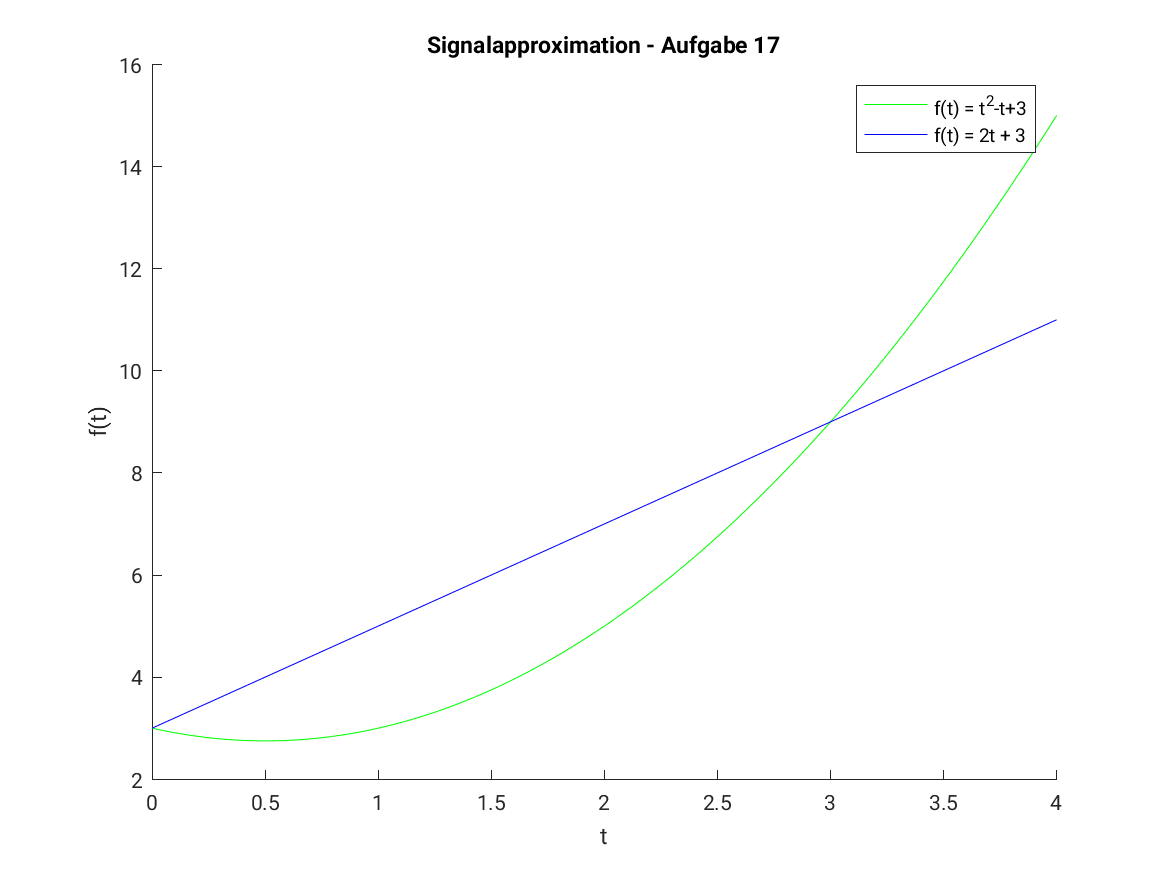
\includegraphics[scale = 0.7]{A17_functionPlot.png}
\end{document}